
\documentclass[tikz, border=1cm]{standalone}
\usepackage{pgfplots}
\pgfplotsset{compat=1.18}
\definecolor{webgreen}{rgb}{0,.5,0}
\definecolor{webblue}{rgb}{0,0,.8}
\definecolor{webred}{rgb}{0.8, 0, 0}   
\definecolor{webbrown}{rgb}{.6,0,0}
\definecolor{webyellow}{rgb}{0.98,0.92,0.73}
\definecolor{webgray}{rgb}{.753,.753,.753}



\begin{document}
	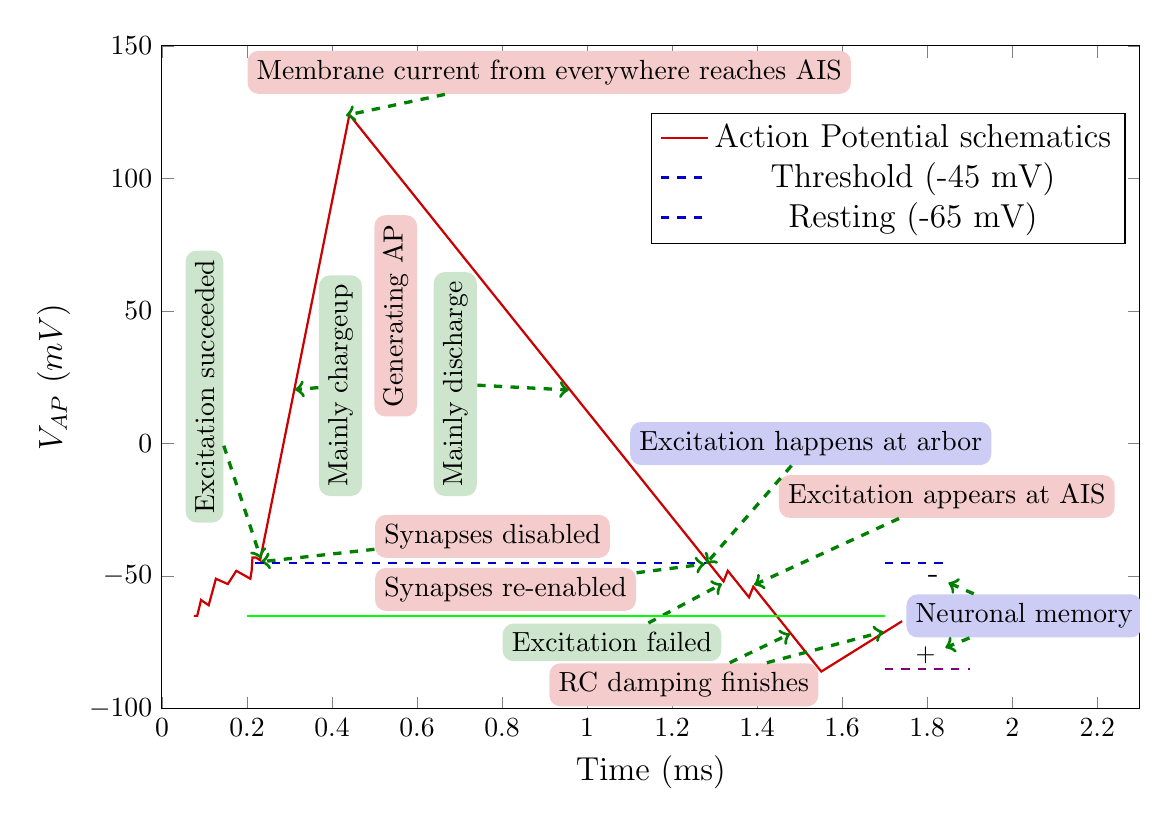
\begin{tikzpicture}
		\begin{axis}[           
		%	hide axis,
			width=14cm, height=10cm,
			xmin=0, xmax=2.3,
			ymin= -100, ymax = 150,
			xlabel={\large Time (ms)},
			ylabel={\large $V_{AP}\ (mV)$},
			legend style={at={(.50,0.80)},anchor=west}
			]


% The main  Action Potential schematics
\addplot[
webred,% thick,
no marks, mark=*, mark size=2, thick,
] plot coordinates {
(  0.075,-65)
(  0.083,-65)
(  0.092,-59)
(  0.110,-61)
(  0.127,-51)
(  0.155,-53)
(  0.175,-48)
(  0.208,-51)
(  0.211,-48)
(  0.213,-43)
(  0.221,-43)
(  0.231,-44)
(  0.241,-36)
(  0.251,-28)
(  0.261,-20)
(  0.271,-12)
(  0.281,-4)
(  0.291,4)
(  0.301,12)
(  0.311,20)
(  0.321,28)
(  0.331,36)
(  0.341,44)
(  0.351,52)
(  0.361,60)
(  0.371,68)
(  0.381,76)
(  0.391,84)
(  0.401,92)
(  0.411,100)
(  0.421,108)
(  0.431,116)
(  0.441,124)
(  0.451,122)
(  0.461,120)
(  0.471,118)
(  0.481,116)
(  0.491,114)
(  0.501,112)
(  0.511,110)
(  0.521,108)
(  0.531,106)
(  0.541,104)
(  0.551,102)
(  0.561,100)
(  0.571,98)
(  0.581,96)
(  0.591,94)
(  0.601,92)
(  0.611,90)
(  0.621,88)
(  0.631,86)
(  0.641,84)
(  0.651,82)
(  0.661,80)
(  0.671,78)
(  0.681,76)
(  0.691,74)
(  0.701,72)
(  0.711,70)
(  0.721,68)
(  0.731,66)
(  0.741,64)
(  0.751,62)
(  0.761,60)
(  0.771,58)
(  0.781,56)
(  0.791,54)
(  0.801,52)
(  0.811,50)
(  0.821,48)
(  0.831,46)
(  0.841,44)
(  0.851,42)
(  0.861,40)
(  0.871,38)
(  0.881,36)
(  0.891,34)
(  0.901,32)
(  0.911,30)
(  0.921,28)
(  0.931,26)
(  0.941,24)
(  0.951,22)
(  0.961,20)
(  0.971,18)
(  0.981,16)
(  0.991,14)
(  1.001,12)
(  1.011,10)
(  1.021,8)
(  1.031,6)
(  1.041,4)
(  1.051,2)
(  1.061,0)
(  1.071,-2)
(  1.081,-4)
(  1.091,-6)
(  1.101,-8)
(  1.111,-10)
(  1.121,-12)
(  1.131,-14)
(  1.141,-16)
(  1.151,-18)
(  1.161,-20)
(  1.171,-22)
(  1.181,-24)
(  1.191,-26)
(  1.201,-28)
(  1.211,-30)
(  1.221,-32)
(  1.231,-34)
(  1.241,-36)
(  1.251,-38)
(  1.261,-40)
(  1.271,-42)
(  1.281,-44)
(  1.291,-46)
(  1.301,-48)
(  1.311,-50)
(  1.321,-52)
(  1.331,-48)
(  1.331,-48)
(  1.341,-50)
(  1.351,-52)
(  1.361,-54)
(  1.371,-56)
(  1.381,-58)
(  1.391,-54)
(  1.391,-54)
(  1.401,-56)
(  1.411,-58)
(  1.421,-60)
(  1.431,-62)
(  1.441,-64)
(  1.451,-66)
(  1.461,-68)
(  1.471,-70)
(  1.481,-72)
(  1.491,-74)
(  1.501,-76)
(  1.511,-78)
(  1.521,-80)
(  1.531,-82)
(  1.541,-84)
(  1.551,-86)
(  1.561,-85)
(  1.571,-84)
(  1.581,-83)
(  1.591,-82)
(  1.601,-81)
(  1.611,-80)
(  1.621,-79)
(  1.631,-78)
(  1.641,-77)
(  1.651,-76)
(  1.661,-75)
(  1.671,-74)
(  1.681,-73)
(  1.691,-72)
(  1.701,-71)
(  1.711,-70)
(  1.721,-69)
(  1.731,-68)
(  1.741,-67)
};
\addlegendentry{\large Action Potential schematics}

       \node[anchor=west, rectangle, rounded corners,fill=webred!20] (sourceC) at (axis cs:0.20,140){Membrane current from everywhere reaches AIS};
		\node (PeakAP) at (axis cs:.41,123){};
		\draw[->,dashed, very thick, webgreen](sourceC)--(PeakAP);


       \node[anchor=west, rectangle, rounded corners,fill=webred!20] (sourceD) at (axis cs:0.50,-35){ Synapses disabled};
		\node (SynapseD) at (axis cs:.21,-45){};
\draw[->,dashed, very thick, webgreen](sourceD)--(SynapseD);

       \node[anchor=west, rectangle, rounded corners,fill=webred!20] (sourceE) at (axis cs:0.50,-55){ Synapses re-enabled};
		\node (SynapseR) at (axis cs:1.30,-45){};
		\draw[->,dashed, very thick, webgreen](sourceE)--(SynapseR);

       \node[anchor=west, rectangle, rounded corners,fill=webgreen!20, rotate=90] (succeded) at (axis cs:0.10,-30){Excitation succeeded};
		\node (Succeeded) at (axis cs:0.24,-47){};
		\draw[->,dashed, very thick, webgreen](succeded)--(Succeeded);


       \node[anchor=west, rectangle, rounded corners,fill=webred!20, rotate=90] (succeded) at (axis cs:0.55,+10){Generating AP};
 
        \node[anchor=west, rectangle, rounded corners,fill=webgreen!20, rotate=90] (Chargeup) at (axis cs:0.420,-20){Mainly chargeup};
		\node (Up) at (axis cs:0.29,20){};
		\draw[->,dashed, very thick, webgreen](Chargeup)--(Up);

        \node[anchor=west, rectangle, rounded corners,fill=webgreen!20, rotate=90] (Discharge) at (axis cs:0.69,-20){Mainly discharge};
		\node (Down) at (axis cs:0.98,20){};
		\draw[->,dashed, very thick, webgreen](Discharge)--(Down);
       
       \node[anchor=west, rectangle, rounded corners,fill=webgreen!20] (failed) at (axis cs:0.8,-75){Excitation failed};
		\node (Failed) at (axis cs:1.34,-51){};
		\draw[->,dashed, very thick, webgreen](failed)--(Failed);

       \node[anchor=west, rectangle, rounded corners,fill=webred!20] (appearsA) at (axis cs:1.45,-20){Excitation appears at AIS};
%		\node (appearsB) at (axis cs:1.31,-50){};
		\node (appearsB) at (axis cs:1.37,-55){};
		\draw[->,dashed, very thick, webgreen](appearsA)--(appearsB);

       \node[anchor=west, rectangle, rounded corners,fill=webblue!20] (happensA) at (axis cs:1.1,0){Excitation happens at arbor};
       
      \node[anchor=west, rectangle, rounded corners,fill=webred!20] (Damping) at (axis cs:0.91,-91){RC damping finishes};
		\node (DampA) at (axis cs:1.50,-70){};
\draw[->,dashed, very thick, webgreen](Damping)--(DampA);
		\node (DampB) at (axis cs:1.72,-70){};
\draw[->,dashed, very thick, webgreen](Damping)--(DampB);
       
       
\node (happensB) at (axis cs:1.26,-49){};
\draw[->,dashed, very thick, webgreen](happensA)--(happensB);

\addplot[
webblue,dashed,
no marks, mark=*, mark size=2, thick,
] plot coordinates {
	(0.22,-45)
	(1.28,-45)
};
\addplot[
webblue,dashed,
no marks, mark=*, mark size=2, thick,
] plot coordinates {
	(1.7,-45)
	(1.85,-45)
};

\addlegendentry{\large Threshold (-45 mV)}
\addplot[
green, thick,
no marks, mark=*, mark size=2, thick,
] plot coordinates {
	(0.2,-65)
	(1.7,-65)
};
\addlegendentry{\large Resting (-65 mV)}

\addplot[
violet,dashed,
no marks, mark=*, mark size=2, thick,
] plot coordinates {
	(1.7,-85)
	(1.9,-85)
};


       \node[anchor=west, rectangle, rounded corners,fill=webblue!20] (memory) at (axis cs:1.75,-65){Neuronal memory};
		\node [below,left] (memoryplus) at (axis cs:1.85,-50){\large -};
		\draw[->,dashed, very thick, webgreen](memory)--(memoryplus);
		\node  [below,right] (memoryminus) at (axis cs:1.75,-80){\small +};
		\draw[->,dashed, very thick, webgreen](memory)--(memoryminus);


		\end{axis}
	
\end{tikzpicture}
\end{document}
	

